\documentclass{article}
\usepackage[utf8]{inputenc}
\usepackage[margin = 0.8in]{geometry}
\usepackage{graphicx}
\usepackage{amsmath, amssymb}
\usepackage{subcaption}
\usepackage{multirow}
\usepackage{mathtools}
\usepackage{float}


\title{RBE549 - Homework 10}
\author{Keith Chester}
\date{Due date: November 23, 2022}

\begin{document}
\maketitle

\section*{Problem 1}

Here we are tasked with finding what velocity $\vec{V}_{MIN}$ satisfies the Optical Flow Constraint Equation (OFCE) $I_x u + I_y v + I_t = 0$ and has the smallest magnitude $|\vec{V}|$.

\begin{figure}[H]
    \centering
    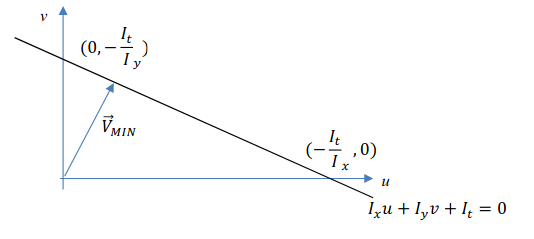
\includegraphics[width = 0.75\textwidth]{imgs/1a.png}
    \caption{Optical Flow Chart}
    \label{fig:3a1}
\end{figure}

To do this, we will first solve for the line between the provided points $(0, -\frac{I_t}{I_y})$ and $(-\frac{I_t}{I_x}, 0)$. From this we can determine the $\vec{V}_{MIN}$ vector. To find the line:

\begin{equation}
    v = mu+b
\end{equation}

\begin{equation}
    -\frac{I_t}{I_y} = m*0 + b
\end{equation}

\begin{equation}
    b = -\frac{I_t}{I_y}
\end{equation}

\noindent ...and now we can solve for $m$:

\begin{equation}
    0 = m (-\frac{I_t}{I_x}) - \frac{I_t}{I_y}
\end{equation}

\begin{equation}
    -\frac{I_t I_x}{I_y I_t} = m
\end{equation}

\begin{equation}
    -\frac{I_x}{I_y} = m
\end{equation}

\noindent ...so our line for the two points is $v = -\frac{I_x}{I_y} u - \frac{I_t}{I_y}$. Since the line perpendicular to a line with slope $m$ is $\frac{-1}{m}$, it follows thats the resulting $m$ for our perpendicular line is thus:

\begin{equation}
    \frac{-1}{m} = \frac{-1}{-\frac{I_x}{I_y}} = \frac{I_y}{I_x}
\end{equation}

\noindent Now we need to find the $b$ for our given line that intersects with $(0,0)$, where our $\vec{V}_{MIN}$ comes from. This suggests that the $b$ is thus $0$, making a final equation

\begin{equation}
    v = \frac{I_y}{I_x} u
\end{equation}

\noindent We then solve for where $\vec{V}_{MIN}$ intersects our line, which would be the minimum velocity required:

\begin{equation}
    \frac{I_y}{I_x} u = -\frac{I_x}{I_y} u - \frac{I_t}{I_y}
\end{equation}

\begin{equation}
    (\frac{I_y}{I_x} + \frac{I_x}{I_y}) u = \frac{I_t}{I_y}
\end{equation}

\begin{equation}
    \frac{I_x^2 + I_y^2}{I_x I_y}u = \frac{I_t}{I_y}
\end{equation}

\begin{equation}
    u = \frac{I_t I_x}{I_x^2 + I_y^2}
\end{equation}

\noindent Now that we know the $u$, we need to find the $v$:

\begin{equation}
    v = \frac{I_y}{I_x} \frac{I_t I_x}{I_x^2 + I_y^2} = \frac{I_t I_y}{I_x^2 + I_y^2}
\end{equation}

\section*{Problem 2}

Here we are told to suppose that a given image's brightness is given by:

\begin{equation}
    I(x,y,t) = I_o + k(tan^{-1}(\frac{x}{y})-st)
\end{equation}

\subsection*{A}

We are tasked with finding $I_x$, $I_y$, $I_t$, which are the partial derivatives of each:

\begin{equation}
    I_x = \frac{k}{y(\frac{x^2}{y^2}+1)} = \frac{k\,y}{x^2 +y^2 }
\end{equation}

\begin{equation}
    I_y = -\frac{kx}{y^2(\frac{x^2}{y^2}+1)} = -\frac{k\,x}{x^2 +y^2 }
\end{equation}

\begin{equation}
    I_t = -ks
\end{equation}

\subsection*{B}

Now, utilizing these partial deriviatives, we wish to find the simplest possible form of $I_x u + I_y v + I_t = 0$. Once we plug in our derivatives, we simplfiy:

\begin{equation}
    \frac{kuy}{x^2 +y^2 }-\frac{kvx}{x^2 +y^2 }-ks=0
\end{equation}

\noindent ...which we can simplify to:

\begin{equation}
    sx^2 +sy^2+vx =uy
\end{equation}

\subsection*{C}

Now we are tasked with showing that the rotating flow field of $u=sy$ and $v=-sx$ is a solution to the OFCE. To do this we'll plug in these values:

\begin{equation}
    \frac{kuy}{x^2 +y^2 }-\frac{kvx}{x^2 +y^2 }-ks=0
\end{equation}

\begin{equation}
    \frac{ksx^2 }{x^2 +y^2 }+\frac{ksy^2 }{x^2 +y^2 }-ks=0
\end{equation}

\begin{equation}
    \frac{sx^2 }{x^2 +y^2 }+\frac{sy^2 }{x^2 +y^2 }-s=0
\end{equation}

\begin{equation}
    \frac{x^2 }{x^2 +y^2 }+\frac{y^2 }{x^2 +y^2 }-1=0
\end{equation}

\begin{equation}
    \frac{x^2 +y^2}{x^2 +y^2 } - 1 =0
\end{equation}

\begin{equation}
    1 - 1 = 0
\end{equation}

\begin{equation}
    0 = 0
\end{equation}

\noindent ...and thus we have proved that these values do solve this OFCE.

\section*{Problem 3}

In this problem we are looking at an iterative method for computing optical flow, with each iteration being updated according to:

\begin{equation}
    \begin{bmatrix}
        u(x,y) \\
        v(x,y)
    \end{bmatrix}^{new} =
    \begin{bmatrix}
        \lambda I_x^2 + 4 & \lambda I_x I_y \\
        \lambda I_x I_y & \lambda I_y^2 + 4
    \end{bmatrix}^{-1}
    \begin{bmatrix}
        \sum_{n\epsilon \textit{neighbors}(x,y)} u^{old}(n)-\lambda I_x I_t \\
        \sum_{n\epsilon \textit{neighbors}(x,y)} v^{old}(n)-\lambda I_y I_t \\
    \end{bmatrix}
\end{equation}

\subsection*{A}

First, we are tasked to show that the equation above is equivalent to 

\begin{equation}
    \begin{bmatrix}
        u(x,y) \\
        v(x,y)
    \end{bmatrix}^{new} =
    \frac{1}{4 \lambda I_x^2 + 4\lambda I_y^2 + 16}
    \begin{bmatrix}
        \lambda I_y^2 + 4 & -\lambda I_x I_y \\
        -\lambda I_x I_y & \lambda I_x^2 + 4
    \end{bmatrix}
    \begin{bmatrix}
        \sum_{n\epsilon \textit{neighbors}(x,y)} u^{old}(n)-\lambda I_x I_t \\
        \sum_{n\epsilon \textit{neighbors}(x,y)} v^{old}(n)-\lambda I_y I_t \\
    \end{bmatrix}
\end{equation}

\noindent The primary difference lies in the second term. First we will define the inverse of a $2x2$ matrix:

\begin{equation}
    \begin{bmatrix}
        a & b \\
        c & d
    \end{bmatrix}^{-1} =
    \frac{1}{ad-bc}
    \begin{bmatrix}
        d & -b \\
        -c & a
    \end{bmatrix}
\end{equation}

\noindent Following this definition, we get:

\begin{equation}
    \begin{bmatrix}
        \lambda I_x^2 + 4 & \lambda I_x I_y \\
        \lambda I_x I_y & \lambda I_y^2 + 4
    \end{bmatrix}^{-1} =
    \frac{1}{(\lambda I_x^2 + 4)(\lambda I_y^2 + 4)- \lambda I_x I_y \lambda I_x I_y}
    \begin{bmatrix}
        \lambda I_y^2 + 4 & -\lambda I_x I_y \\
        -\lambda I_x I_y & \lambda I_y^2 + 4
    \end{bmatrix}
\end{equation}

\noindent ...which simplifies to:

\begin{equation}
    \frac{1}{4 \lambda I_x^2 + 4\lambda I_y^2 + 16}
    \begin{bmatrix}
        \lambda I_y^2 + 4 & -\lambda I_x I_y \\
        -\lambda I_x I_y & \lambda I_x^2 + 4
    \end{bmatrix}
\end{equation}

\noindent ...which thus proves the two equations are equivalent.

\subsection*{B}

We are then tasked with showing that this is the equivalent to the update equations:

\begin{equation}
    u^{new}(x,y) = \bar{u}^{old}-\frac{I_x}{I_x^2+I_y^2+\frac{4}{\lambda}(I_x\bar{u}^old}+I_t)
\end{equation}

\begin{equation}
    v^{new}(x,y) = \bar{v}^{old}-\frac{I_y}{I_x^2+I_y^2+\frac{4}{\lambda}(I_x\bar{u}^old}+I_t)
\end{equation}

\noindent ...where $\bar{u}^{old}$ and $\bar{v}^{old}$ are the averages of the 4 neighbors of $u(x,y)$ and $v(x,y)$.

\noindent First, we further define $\bar{u}^{old}$ mathematically:

\begin{equation}
    \bar{u}^{old} = \frac{1}{4} \Sigma_{n\epsilon \textit{neighbors}(x,y)} u^{old}(n)
\end{equation}

\begin{equation}
    4\bar{u}^{old} = \Sigma_{n\epsilon \textit{neighbors}(x,y)} u^{old}(n)
\end{equation}

\noindent ...so if we looked at our base equation now:

\begin{equation}
    u^{new}(x,y) =
    \frac{1}{4(\lambda I_x^2 + \lambda I_y^2 + 4)}
    \begin{bmatrix}
        \lambda I_y^2 + 4 & -\lambda I_x I_y
    \end{bmatrix}
    \begin{bmatrix}
        4\bar{u}^{old}-\lambda I_x I_t \\
        4\bar{v}^{old}-\lambda I_y I_t \\
    \end{bmatrix}
\end{equation}

\noindent We can then expand this out by performing vector multiplication, getting:

\begin{equation}
    u^{new}(x,y) = \frac{1}{4(\lambda I_x^2 + \lambda I_y^2 + 4)}
    \big(
    (\lambda I_y^2 +4)(4\bar{u}^{old}-\lambda I_x I_t) - (\lambda I_x I_y)(4\bar{v}^{old}+\lambda I_x I_y \lambda I_y I_t)
    )
\end{equation}

\noindent We can expand this:

\begin{equation}
    u^{new}(x,y) = \frac
    {\lambda I_y^2 4\bar{u}^{old}-\lambda I_y^2 \lambda I_x I_t + 16\bar{u}^{old}-4\lambda I_x I_t-(\lambda I_x I_y)4\bar{v}^{old}+\lambda^2 I_y^2 I_x I_t}
    {4(\lambda I_x^2 + \lambda I_y^2 + 4)}
\end{equation}

\begin{equation}
    u^{new}(x,y) = \frac
    {4(\lambda I_y^2 \bar{u}^{old} - \lambda I_x I_t - \lambda I_x I_y \bar{v}^{old})}
    {4(\lambda I_x^2 + \lambda I_y^2 + 4)}
\end{equation}

\begin{equation}
    u^{new}(x,y) = \frac
    {(\lambda I_y^2 \bar{u}^{old} - \lambda I_x I_t - \lambda I_x I_y \bar{v}^{old})}
    {(\lambda I_x^2 + \lambda I_y^2 + 4)}
\end{equation}

\begin{equation}
    u^{new}(x,y) = \frac
    {\bar{u}^{old} (\lambda I_y^2 + 4) - \lambda I_x (I_t + I_y \bar{v}^{old})}
    {\lambda (I_x^2 + I_y^2 + \frac{4}{\lambda})}
\end{equation}

\noindent Here we can add some terms that help us reduce complexity in the numerator after factoring:

\begin{equation}
    u^{new}(x,y) = \frac
    {\lambda I_y^2 \bar{u}^{old} - \lambda I_x I_t - \lambda I_x I_y \bar{v}^{old} + \lambda I_x^2 \bar{u}^{old}-\lambda I_x^2 \bar{u}^{old}}
    {\lambda (I_x^2 + I_y^2 + \frac{4}{\lambda})}
\end{equation}

\begin{equation}
    u^{new}(x,y) = \frac
    {\bar{u}^{old}\lambda(I_y^2 +  I_x^2 + \frac{4}{\lambda}) - \lambda I_x^2 - \bar{u}^{old} - \lambda I_x I_t - \lambda I_x I_y \bar{v}^{old}}
    {\lambda (I_x^2 + I_y^2 + \frac{4}{\lambda})}
\end{equation}

\begin{equation}
    u^{new}(x,y) = \bar{u}^{old} - \frac
    {\lambda I_x^2 \bar{u}^{old} - \lambda I_x I_t - \lambda I_x I_y \bar{v}^{old}}
    {\lambda (I_x^2 + I_y^2 + \frac{4}{\lambda})}
\end{equation}

\begin{equation}
    u^{new}(x,y) = \bar{u}^{old} - \lambda I_x \Bigg(\frac
    {I_x \bar{u}^{old} + I_y \bar{v}^{old} + I_t}
    {\lambda (I_x^2 + I_y^2 + \frac{4}{\lambda})}\Bigg)
\end{equation}

\begin{equation}
    u^{new}(x,y) = \bar{u}^{old} -
    \frac{I_x}{I_x^2 + I_y^2 + \frac{4}{\lambda}}
    \bigg(
        I_x \bar{u}^{old} + I_y \bar{v}^{old} + I_t
    \bigg)
\end{equation}


\noindent And with this, we can presume that the update equation for $v^{new}$ is similarly:

\begin{equation}
    v^{new}(x,y) = \bar{v}^{old} -
    \frac{I_x}{I_x^2 + I_y^2 + \frac{4}{\lambda}}
    \bigg(
        I_x \bar{u}^{old} + I_y \bar{v}^{old} + I_t
    \bigg)
\end{equation}


\subsection*{C}

Here we are tasked with finding out what the update equations found above reduce to when $\lambda = 0$.

\begin{equation}
    u^{new}(x,y) = \bar{u}^{old} -
    \frac{I_x}{I_x^2 + I_y^2 + \frac{4}{\lambda}}
    \bigg(
        I_x \bar{u}^{old} + I_y \bar{v}^{old} + I_t
    \bigg)
\end{equation}

We have to adjust the denominator I showed above, because we wish to avoid the undefined nature the $\frac{4}{\lambda}$ introduces. Thus we multiply by $\frac{\lambda}{\lambda}$.

\begin{equation}
    u^{new}(x,y) = \bar{u}^{old} -
    \frac{\lambda I_x}{\lambda I_x^2 + \lambda I_y^2 + 4}
    \bigg(
        I_x \bar{u}^{old} + I_y \bar{v}^{old} + I_t
    \bigg)
\end{equation}

\noindent ...and replaceing $\lambda=0$ yields:

\begin{equation}
    u^{new}(x,y) = \bar{u}^{old} -
    \frac{0 * I_x}{0 * I_x^2 + 0 * I_y^2 + 4}
    \bigg(
        I_x \bar{u}^{old} + I_y \bar{v}^{old} + I_t
    \bigg)
\end{equation}

\begin{equation}
    u^{new}(x,y) = \bar{u}^{old} -
    \frac{0}{4}
    \bigg(
        I_x \bar{u}^{old} + I_y \bar{v}^{old} + I_t
    \bigg)
\end{equation}

\begin{equation}
    u^{new}(x,y) = \bar{u}^{old}
\end{equation}

\noindent ...and it goes to follow that for $v^{new}(x,y)= \bar{v}^{old}$ is for our $v$ update equation.


\end{document}